\documentclass[]{article}
\usepackage[utf8]{inputenc}
\usepackage{graphicx}
\usepackage{textcomp}
\usepackage{fullpage}
\usepackage{float}
\usepackage{listings}
\usepackage{verbatim}

\title{Deep Learning Assignment 3}
\author{Nikita Teplitskiy}

\begin{document}
\maketitle
\section{Introduction}
This assignment was completed with TensorFlow using a two layer perceptron. The completed model achieves a 95.99\% accuracy on the provided test dataset and a 95.63\% accuracy on the validation subset. It uses a total of 14,320 trainable parameters. As part of the assignment, a custom data loader titled ``MNISTload.py'' was developed and is provided below.

\begin{figure}[H]
    \centering
    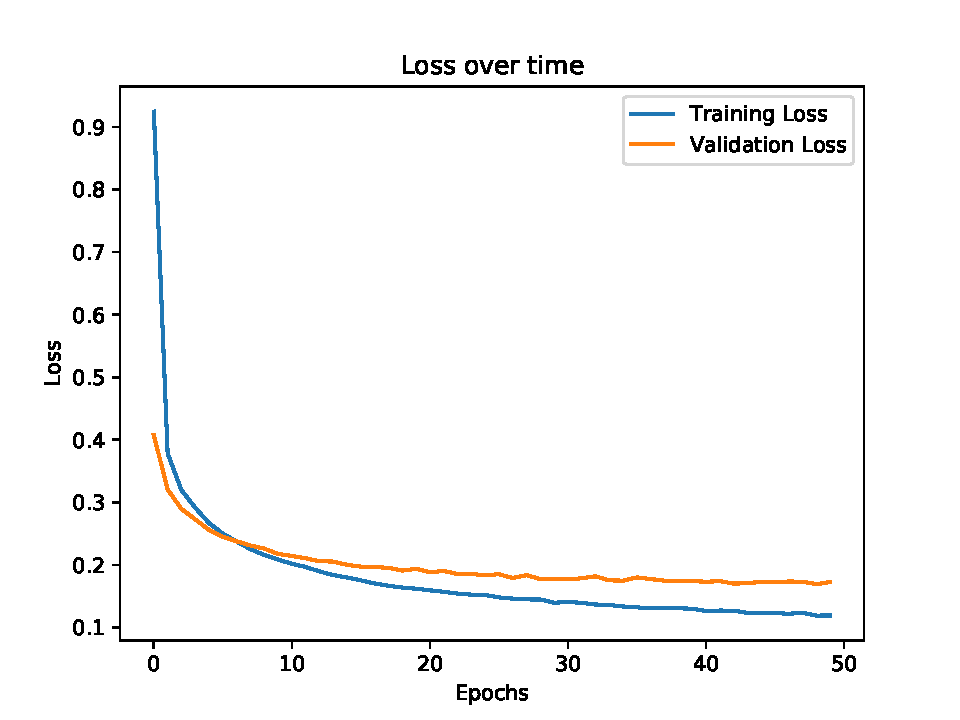
\includegraphics[width=0.6\textwidth]{loss.pdf}
    \caption{Loss over training iterations}
\end{figure}

\noindent
From the loss plot one can see that the validation loss begins to exceed the training loss within the first 10 epochs. This suggests a degree of overfitting and increased regularization would be required to fix this. This was not done as the desired accuracy had been achieved. 

\newpage
\onecolumn
%\verbatiminput{a2.py}

\newpage
\section{Model}
\lstinputlisting[language=Python]{a3.py}

\newpage
\section{Data Loader}
\lstinputlisting[language=Python]{MNISTload.py}

\end{document}
